\documentclass[oneside]{report}
\usepackage[T1]{fontenc}
\usepackage[utf8]{inputenc}
\usepackage[french]{babel}
\usepackage{graphicx}
\usepackage[margin=2cm]{geometry}
\usepackage{fancyhdr}
\usepackage{changepage}
\usepackage{etoolbox}
\usepackage{xcolor}
\usepackage{titlesec}

\titleformat{\chapter}[display]
{\normalfont\huge\bfseries}{}{20pt}{\Huge}

\titlespacing*{\chapter}{0pt}{0pt}{0pt}
\graphicspath{{./images/}}

\author{Sylvain COMBRAQUE, Sarah LAMOTTE, Nathan JANCZEWSKI, Léo BERGEROT}

\newcommand\softname{Alohomora\ }
\newcommand{\writecol}[1]{
	\subitem{\textcolor[HTML]{#1}{\# #1}}
}

\patchcmd{\chapter}{plain}{fancy}{}{}

\begin{document}

	\begin{titlepage}
		\centering
		
\includegraphics[scale=.5]{logo_large}
		\vspace{5cm}
		{\par\scshape\Huge Cahier des charges\par}
		\vspace{5cm}
		{\par Gestionnaire de mot de passes\par}
		{\par Application et API\par}
		\vfill
		\par Contact:
		{\par\small Mr.\ Jerôme CUTRONA \par}
		\par jerome.cutrona@univ-reims.fr\
	\end{titlepage}

	\pagestyle{fancy}
	\fancyhf{}
	\rhead{
\includegraphics[scale=.25]{logo_large}}
	\lhead{Cahier des charges}
	\tableofcontents

	\chapter{Présentation du projet}
	\vspace{2cm}
	\par Ce projet pour le quatrième semestre du DUT Informatique a pour but de créer un gestionnaire de mot de passe.
	\vspace{.5cm}
	\par Un gestionnaire de mot de passe est un logiciel permettant de n'avoir à retenir qu'un seul mot de passe pour tous ses comptes, le tout sans compromettre leur sécurité. Pour cela, il va générer des mots de passe qui ne seront pas à retenir par l'utilisateur à l'exception du "mot de passe maître" qui permet alors leur chiffrement.
	\vspace{.5cm}
	\par Bien évidemment, la sécurité du logiciel repose sur le fait que l'utilisateur choisisse un mot de passe suffisament fort dès le début, mais délesté de devoir retenir tous les différents mots de passe pour différents sites, il peut alors en retenir un seul plus conséquent.
	\vspace{.5cm}
	\par Contrairement aux alternatives opensources telles que KeePass ou Encryptr, \softname permettera l'utilisation d'un compte relié à un serveur afin que l'utilisateur n'ait pas à gérer le fichier contenant les mots de passes et puisse se connecter de n'importe quelle machine sans attendre la synchronisation via de tiers services.

	\vspace{.5cm}
	\par De plus, l'application sera aussi bien disponible dans un navigateur (Ordinateur, tablette, téléphone) qu'en application smartphone afin de faciliter l'usage.

	\newpage

	\section{Comité de pilotage}
	{
		\par L'équipe gérant le projet utilise la méthode \textit{SCRUM}. Ainsi, le développement est découpé en \textit{sprints}, période pouvant aller d'une à trois semaines, les membres de l'équipe commencenront par définir les fonctionnalités à implémenter, les développeront puis le sprint se concluera par une démonstration au client, qui pourra alors vérifier le respect du cahier des charges.
		\vspace{.5cm}
		\par Le client peut aussi demander s'il le souhaite une validation de l'ergonomie, qui sera effectuée en testant l'application sur diverses personnes externes n'étant pas du domaine de l'informatique.
	}

	\section{Objectifs de l'application}
	{
		\par L'application a pour but de stocker les mot de passes des utilisateurs l'utilisant. Cependant, l'utilisateur pourra aussi stocker d'autres informations, telles que des mémos ou des favoris internet.
		\vspace{.5cm}
		\par Afin d'être sécurisé, l'hébergeur ne doit pas pouvoir savoir quels sont les différentes informations stockées par l'utilisateur sur le serveur, ainsi un chiffrement total des données transitant vers l'hébergeur et y résidant devra être effectué via un algorithme symétrique, le tout ne dévoilant pas la clé à la personne chargée de l'hébergement.
	}

	\section{Les cibles (À qui s'adresse l'application)}
	{
		\par L'application vise deux types de personnes:
		\begin{itemize}
			\item Les néophytes \par Ces derniers ne voulant simplement qu'utiliser le gestionnaire de mot de passes peuvent alors utiliser une version hébergée par un tiers de l'application.
			\item Les confirmés \par Ceux-ci préfèrent héberger leur propre serveur afin de ne pas dépendre d'un tiers et de ne pas avoir à faire confiance à un hébergeur (Même si le fonctionnement de l'application ne doit pas laisser ce dernier en connaissance des éléments stockés par l'utilisateur)
		\end{itemize}
	}

	\section{Langues}
	{
		\par Un simple système de traduction sera mis en place afin de laisser la possibilité à l'utilisateur de sélectionner la langue dans laquelle il est le plus à l'aise.
		\par La traduction sera faite via un simple fichier de propriétés classique.
	}

	\section{Maquette}
	{
		\par Connexion:\\
		\noindent\makebox[\textwidth]{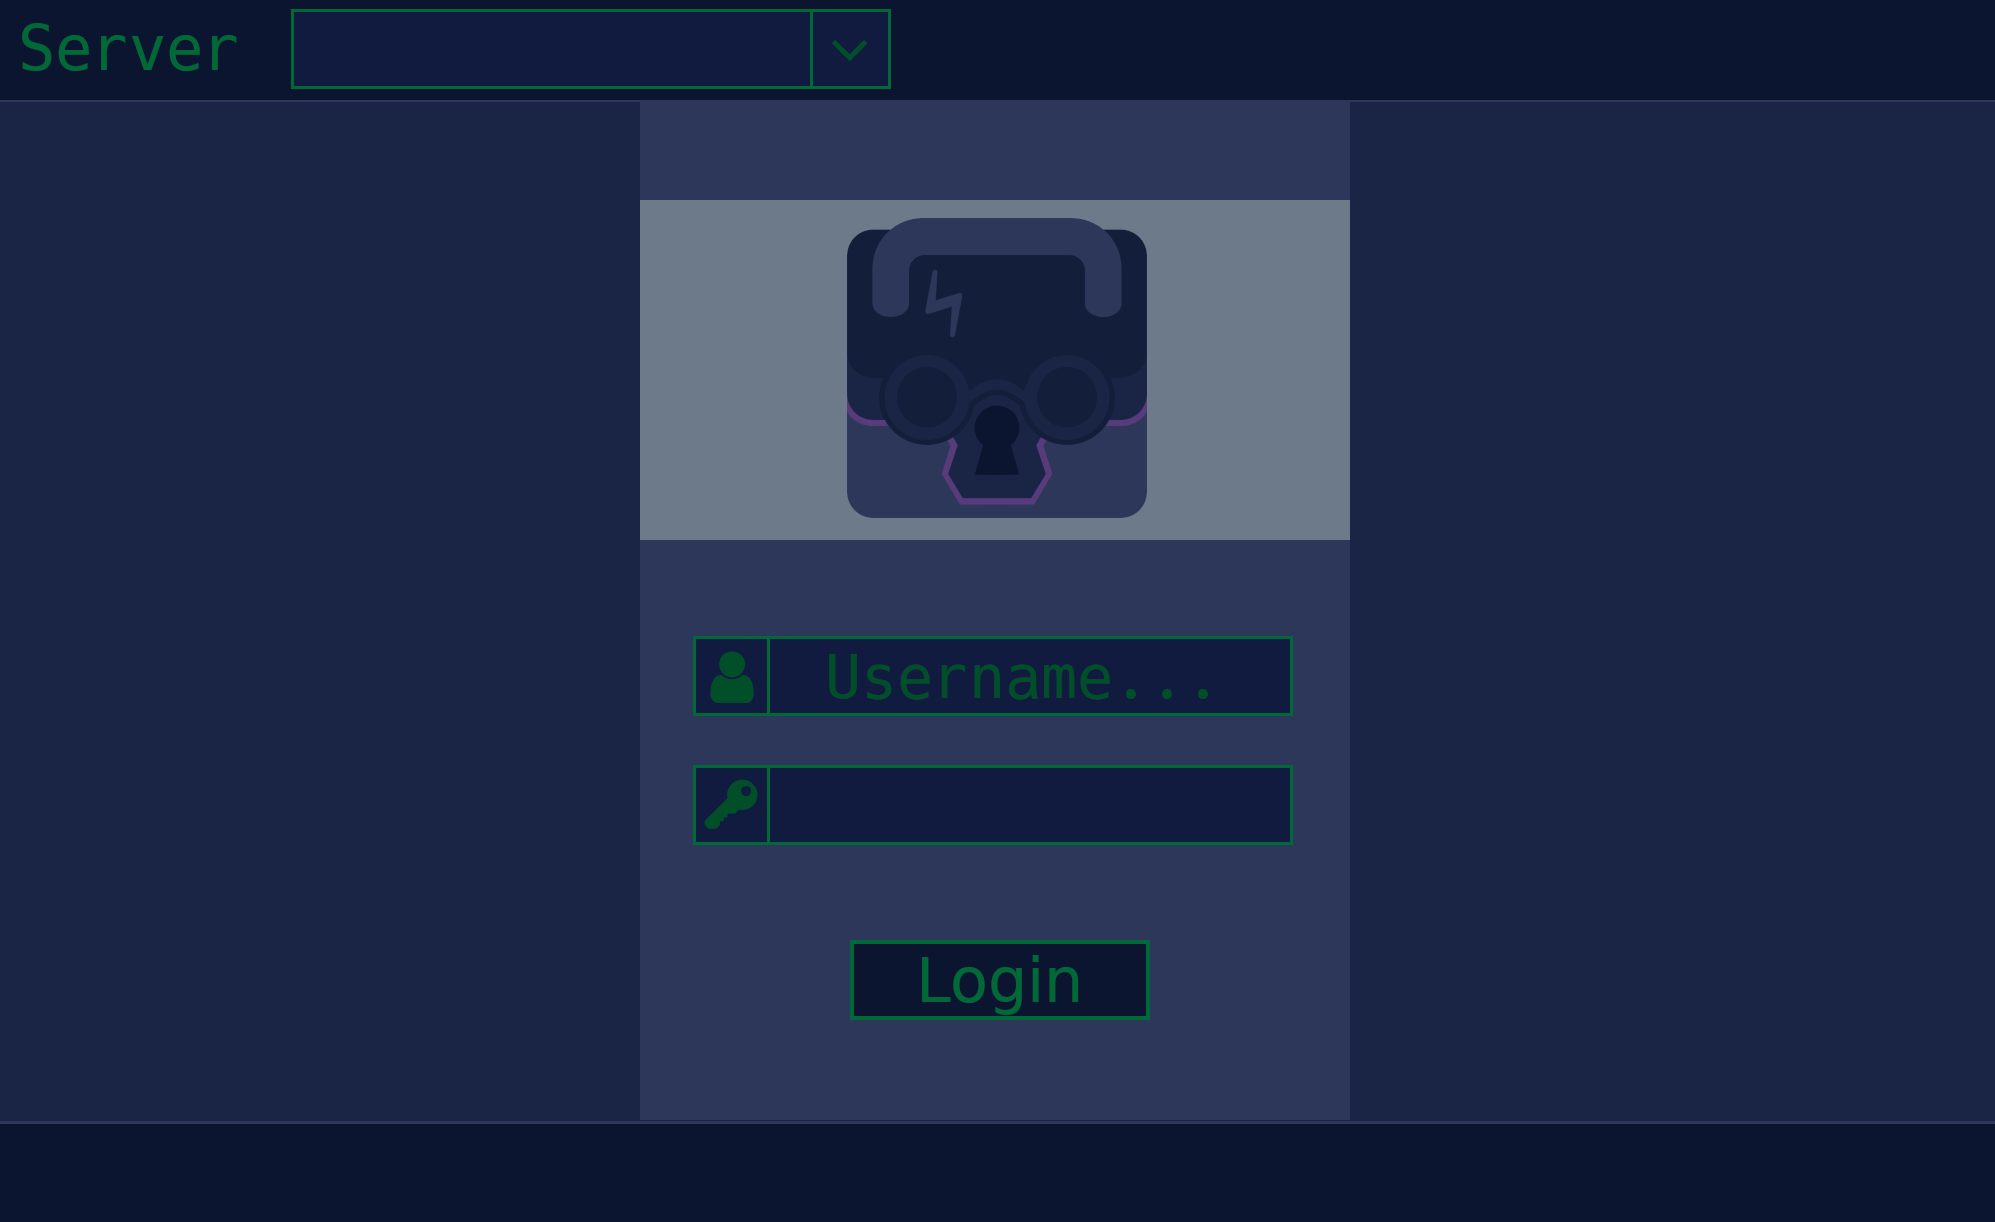
\includegraphics[scale=.5]{maquette_login}}
		\par Fenêtre principale:\\
		\noindent\makebox[\textwidth]{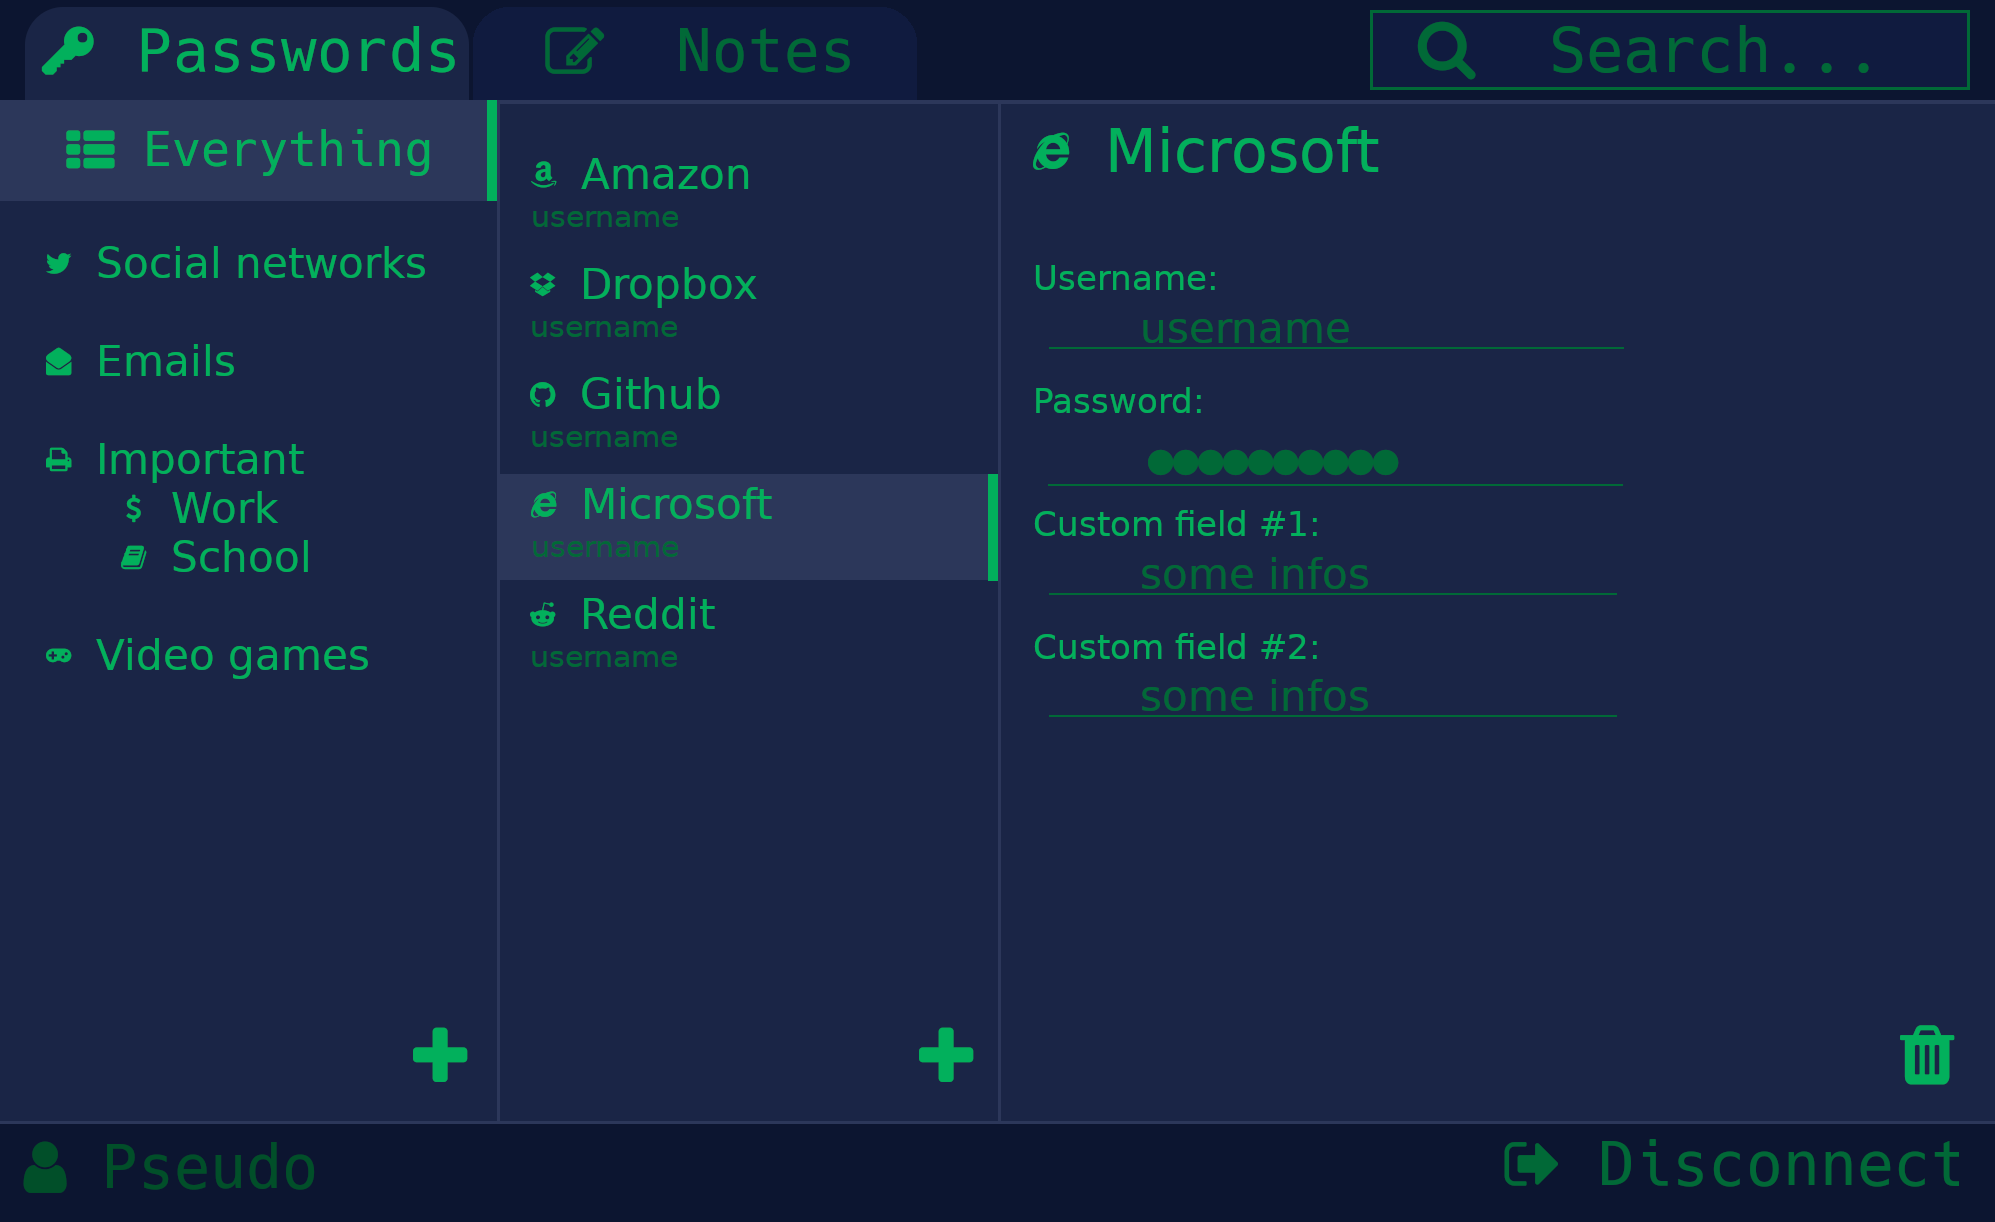
\includegraphics[scale=.5]{maquette_app}}
	}

	\section{Schéma d'utilisation}
	{
		\noindent\makebox[\textwidth]{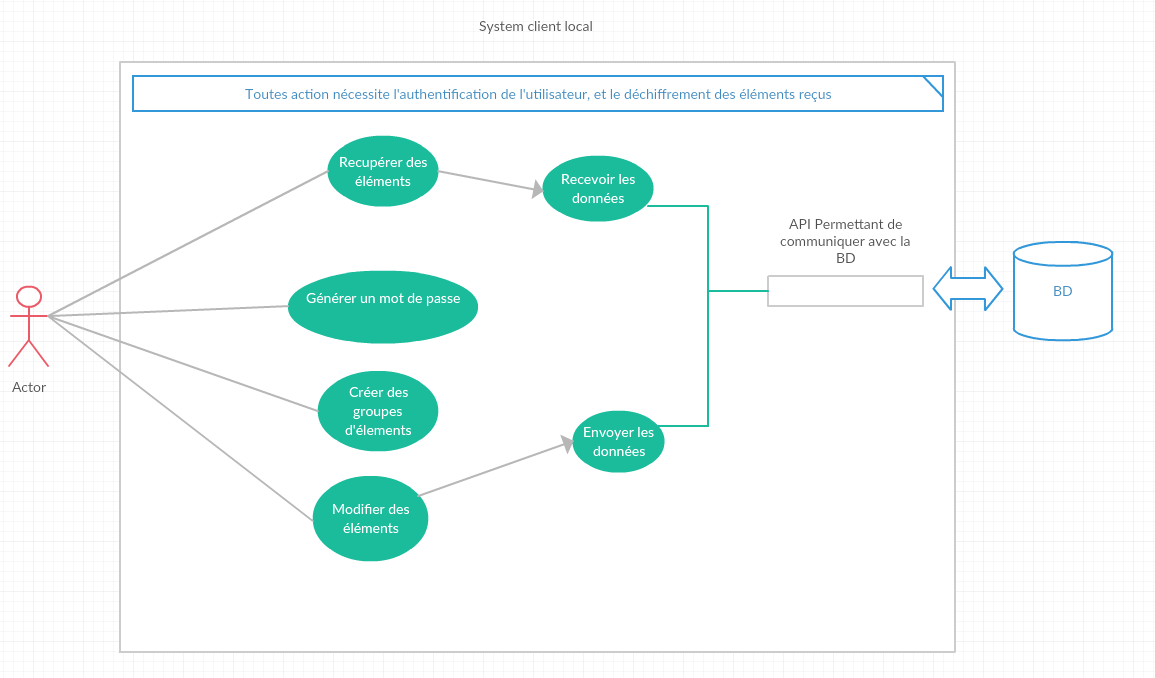
\includegraphics[scale=.5]{usecase}}
	}
	\newpage

	\section{Fonctionnalités}
	{
		\begin{itemize}
			\item Système de comptes
			\item Inscription
			\item Sélection du serveur sur lequel on est inscrit (URL)
			\item Possibilité d'enregistrer des notes
			\item Possibilité d'enregistrer des URL (Marque-Pages)
			\item Groupes d'éléments (Mots de passe, Mémos, Marques-pages)
			\item Génération de mots de passe aléatoire
		\end{itemize}
	}

	\chapter{Prestations attendues}

	\section{Charte graphique}
	{
		\par La charte graphique est la suivante:\\
		\begin{itemize}
			\item Couleurs:
				\writecol{0C1530}
				\writecol{131e3b}
				\writecol{1A2546}
				\writecol{573b7a}
				\writecol{2C375A}
				\writecol{016937}
				\writecol{06a75b}\\
			\item Typographie: Hack patchée avec NerdFont pour les icones\\
			\item{Logo:}\\
				\par
\includegraphics[scale=.125]{logo}
		\end{itemize}
	}

	\section{Hébergement}
	{
		\par Le projet sera hébergé sur un serveur personnel.
		\par Il sera accessible via nom de domaine \textit{https://alohomora.pw/}.
		\par Le domaine de premier niveau choisi étant une référence à "\textbf{p}ass\textbf{w}ord"
	}

	\chapter{Développement}
	\par Le projet est décomposé en plusieurs parties:
	\begin{itemize}
		\item \par Une API Web codée en Symfony 4 reposant sur un serveur MySQL pour la gestion des données utilisateur.\\
		\item \par Un client JavaFX pour le logiciel principal\\
		\item \par En fonction du temps disponible, un client Web (ReactJS) et un client smartphone (React Native) seront créés.
	\end{itemize}
	\section{Base de donnée}
	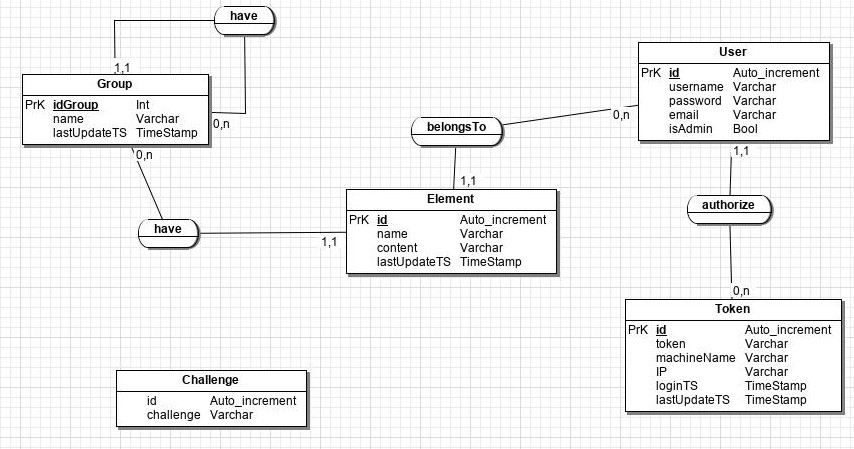
\includegraphics[scale=2]{mcd}

	\section{User stories}
	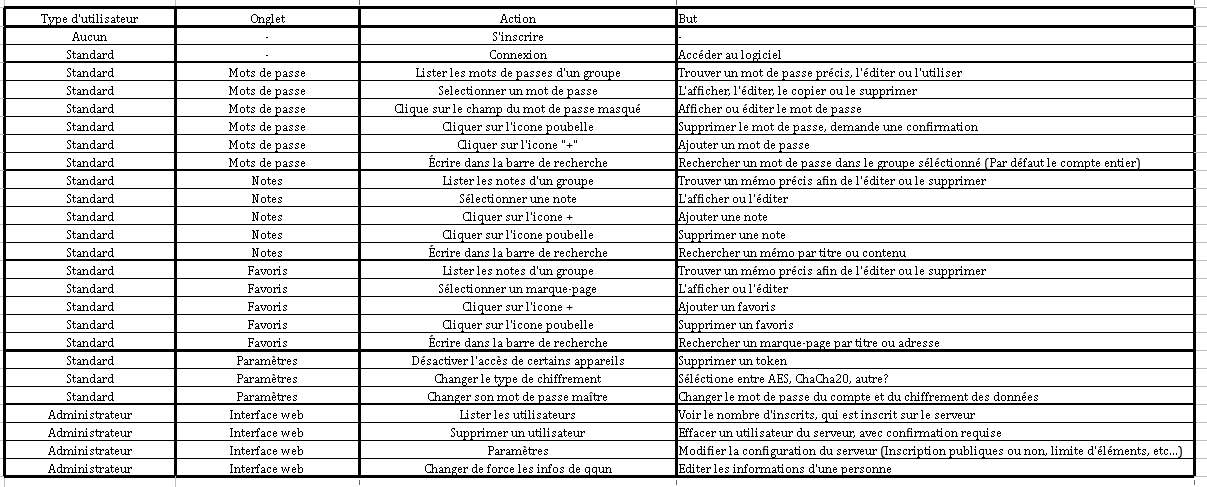
\includegraphics[scale=.40]{userstories}

	\chapter{Planning prévisionnel}
	\par L'utilisation de la méthode agile \textit{SCRUM} implique que nous recueillerons les fonctions essentielles à partir du cahier des charges et des users stories, par conséquent nous écrirons des \textit{backlogs} du produit (liste des fonctionnalités) qui seront classées par priorité, permettant de définir l'ordre de réalisation et ensuite les \textit{sprints} seront réalisés avec toute l'équipe de développement en décidant du sous-ensemble qui sera à réaliser à chaque fois.

	\chapter{Budget}
	\par Étant un projet universitaire, aucun budget n'est alloué à la création du projet.

\end{document}
